% autosam.tex
% Annotated sample file for the preparation of LaTeX files
% for the final versions of papers submitted to or accepted for 
% publication in AUTOMATICA.

% See also the Information for Authors.

% Make sure that the zip file that you send contains all the 
% files, including the files for the figures and the bib file.

% Output produced with the elsart style file does not imitate the
% AUTOMATICA style. The style file is generic for all Elsevier
% journals and the output is laid out for easy copy editing. The
% final document is produced from the source file in the
% AUTOMATICA style at Elsevier.

% You may use the style file autart.cls to obtain a two-column 
% document (see below) that more or less imitates the printed 
% Automatica style. This may helpful to improve the formatting 
% of the equations, tables and figures, and also serves to check 
% whether the paper satisfies the length requirements.

% Please note: Authors must not create their own macros.

% For further information regarding the preparation of LaTeX files 
% for Elsevier, please refer to the "Full Instructions to Authors" 
% from Elsevier's anonymous ftp server on ftp.elsevier.nl in the
% directory pub/styles, or from the internet (CTAN sites) on
% ftp.shsu.edu, ftp.dante.de and ftp.tex.ac.uk in the directory
% tex-archive/macros/latex/contrib/supported/elsevier.


%\documentclass{elsart}               % The use of LaTeX2e is preferred.

\documentclass[twocolumn]{autart}    % Enable this line and disable the 
                                     % preceding line to obtain a two-column 
                                     % document whose style resembles the
                                     % printed Automatica style.


\usepackage{graphicx}          % Include this line if your 
                               % document contains figures,
%\usepackage[dvips]{epsfig}    % or this line, depending on which
                               % you prefer.

\begin{document}

\begin{frontmatter}
%\runtitle{Insert a suggested running title}  % Running title for regular 
                                              % papers but only if the title  
                                              % is over 5 words. Running title 
                                              % is not shown in output.

\title{In Catilinam IV\thanksref{footnoteinfo}} % Title, preferably not more 
                                                % than 10 words.

\thanks[footnoteinfo]{This paper was not presented at any IFAC 
meeting. Corresponding author M.~T.~Cicero. Tel. +XXXIX-VI-mmmxxi. 
Fax +XXXIX-VI-mmmxxv.}

\author[Paestum]{Marcus Tullius Cicero}\ead{cicero@senate.ir},    % Add the 
\author[Rome]{Julius Caesar}\ead{julius@caesar.ir},               % e-mail address 
\author[Baiae]{Publius Maro Vergilius}\ead{vergilius@culture.ir}  % (ead) as shown

\address[Paestum]{Buckingham Palace, Paestum}  % Please supply                                              
\address[Rome]{Senate House, Rome}             % full addresses
\address[Baiae]{The White House, Baiae}        % here.

          
\begin{keyword}                           % Five to ten keywords,  
Cicero; Catiline; orations.               % chosen from the IFAC 
\end{keyword}                             % keyword list or with the 
                                          % help of the Automatica 
                                          % keyword wizard


\begin{abstract}                          % Abstract of not more than 200 words.
Cum M.~Cicero consul Nonis Decembribus senatum in aede Iovis 
Statoris consuleret, quid de iis coniurationis Catilinae sociis 
fieri placeret, qui in custodiam traditi essent, factum est, ut 
duae potissimum sententiae proponerentur, una D.~Silani consulis 
designati, qui morte multandos illos censebat, altera C.~Caesaris, 
qui illos publicatis bonis per municipia Italiae distribuendos 
ac vinculis sempiternis tenendos existimabat.
\end{abstract}

\end{frontmatter}

\section{Introduction}
Video, patres conscripti, in me omnium vestrum ora atque oculos esse 
conversos, video vos non solunn de vestro ac rei publicae, verum 
etiam, si id depulsum sit, de meo periculo esse sollicitos. Est mihi 
iucunda in malis et grata in dolore vestra erga me voluntas, sed eam, 
per deos inmortales, deponite atque obliti salutis meae de vobis ac 
de vestris liberis cogitate. Mihi si haec condicio consulatus data 
est, ut omnis acerbitates, onunis dolores cruciatusque perferrem, 
feram non solum fortiter, verum etiam lubenter, dum modo meis 
laboribus vobis populoque Romano dignitas salusque pariatur.

\begin{figure}
\begin{center}
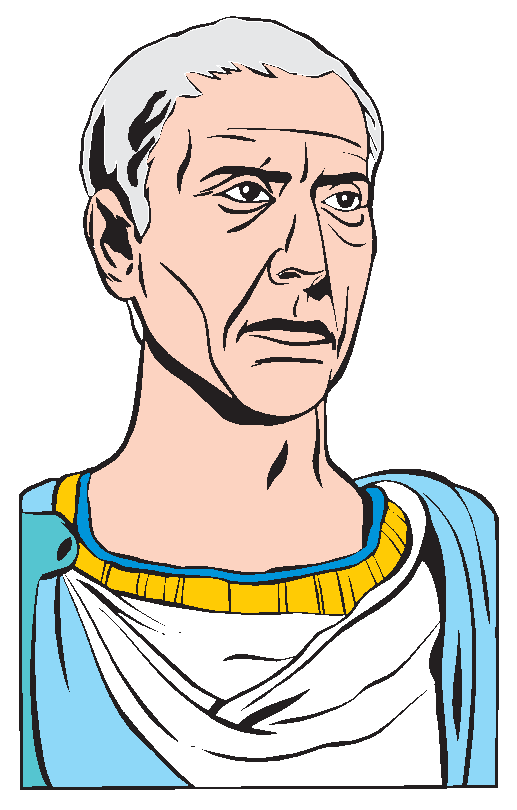
\includegraphics[height=4cm]{jcaesar.eps}    % The printed column  
\caption{Gaius Julius Caesar, 100--44 B.C.}  % width is 8.4 cm.
\label{fig1}                                 % Size the figures 
\end{center}                                 % accordingly.
\end{figure}

% OR

%\begin{figure}
%\begin{center}
%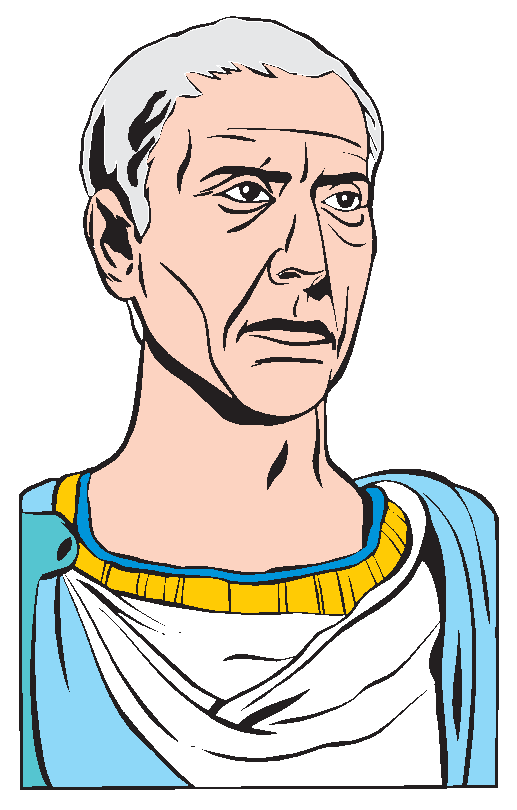
\epsfig{file=jcaesar,width=7cm}
%\caption{Gaius Julius Caesar, 100--44 B.C.}
%\label{fig1}
%\end{center}
%\end{figure}


\subsection{A subsection}
Marcus Tullius Cicero, 106--43 B.C. was a Roman statesman, orator, 
and philosopher.  A major figure in the last years of the Republic, 
he is best known for his orations against Catiline\footnote{
This footnote should be very brief.}
and for his mastery of Latin prose \cite{Heritage:92}. He was a 
contemporary of Julius Caesar (Fig.~\ref{fig1}).

\section{The argument}
Some words might be appropriate describing equation~(\ref{e1}), if 
we had but time and space enough.
\begin{equation} \label{e1}
{{\partial F}\over {\partial t}} =
D{{\partial^2 F}\over {\partial x^2}}.
\end{equation}
See \cite{Abl:56}, \cite{AbTaRu:54}, \cite{Keo:58} and 
\cite{Pow:85}.
This equation goes far beyond the celebrated theorem ascribed to the great
Pythagoras by his followers.
\begin{thm}
The square of the length of the hypotenuse of a right triangle equals the sum of the squares 
of the lengths of the other two sides.
\end{thm}
\section{Epilogue}
A word or two to conclude, and this even includes some inline 
maths:  $R(x,t)\sim t^{-\beta}g(x/t^\alpha)\exp(-|x|/t^\alpha)$.

\begin{ack}                               % Place acknowledgements
Partially supported by the Roman Senate.  % here.
\end{ack}

\bibliographystyle{plain}        % Include this if you use bibtex 
\bibliography{autosam}           % and a bib file to produce the 
                                 % bibliography (preferred). The
                                 % correct style is generated by
                                 % Elsevier at the time of printing.

%\begin{thebibliography}{99}     % Otherwise use the  
                                 % thebibliography environment.
                                 % Insert the full references here.
                                 % See a recent issue of Automatica 
                                 % for the style.
%  \bibitem[Heritage, 1992]{Heritage:92}
%     (1992) {\it The American Heritage. 
%     Dictionary of the American Language.}
%     Houghton Mifflin Company.
%  \bibitem[Able, 1956]{Abl:56}
%     B.~C.~Able (1956). Nucleic acid content of macroscope. 
%     {\it Nature 2}, 7--9. 
%  \bibitem[Able {\em et al.}, 1954]{AbTaRu:54}   
%     B.~C. Able, R.~A. Tagg, and M.~Rush (1954).
%     Enzyme-catalyzed cellular transanimations.
%     In A.~F.~Round, editor, 
%     {\it Advances in Enzymology Vol. 2} (125--247). 
%     New York, Academic Press.
%  \bibitem[R.~Keohane, 1958]{Keo:58}
%     R.~Keohane (1958).
%     {\it Power and Interdependence: 
%     World Politics in Transition.}
%     Boston, Little, Brown \& Co.
%  \bibitem[Powers, 1985]{Pow:85}
%     T.~Powers (1985).
%     Is there a way out?
%     {\it Harpers, June 1985}, 35--47.

%\end{thebibliography}

\appendix
\section{A summary of Latin grammar}    % Each appendix must have a short title.
\section{Some Latin vocabulary}         % Sections and subsections are supported  
                                        % in the appendices.
\end{document}